\chapter{Titulo Capítulo}
	
\lipsum[1-6]
	
\begin{figure}[!h]
	\begin{subfigure}{\linewidth}
		\caption{Titulo}\label{fig:test}
		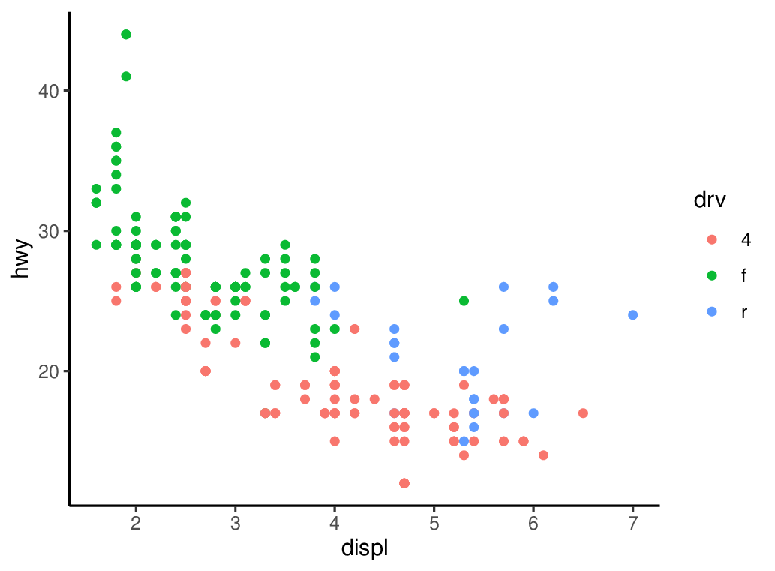
\includegraphics{fig/plot}
		\source{mpg, EUA}
		\notes{Mais observações}
	\end{subfigure}
	\begin{subfigure}{\linewidth}
		\caption{Titulo}
		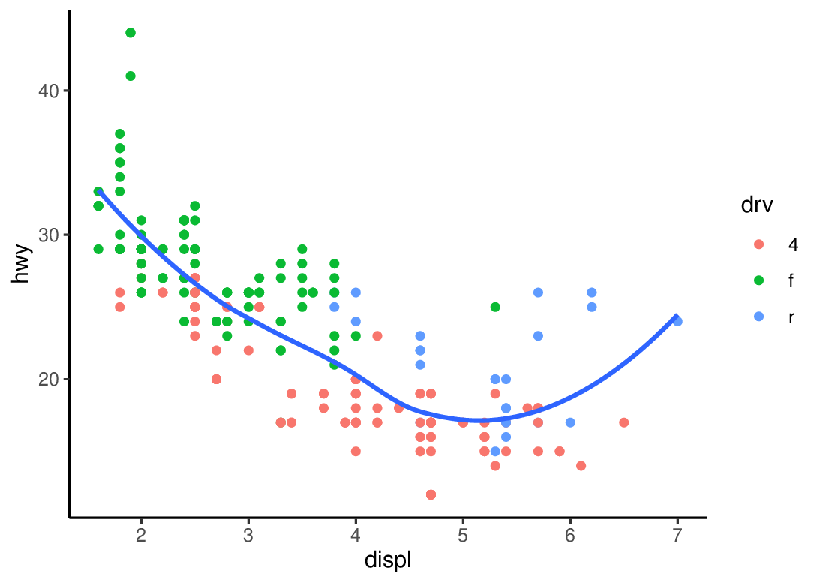
\includegraphics{fig/plot2}
		\source{mpg, EUA}
		\notes{Mais observações}
	\end{subfigure}
	\begin{subfigure}{\linewidth}
		\subcaption{Titulo}
		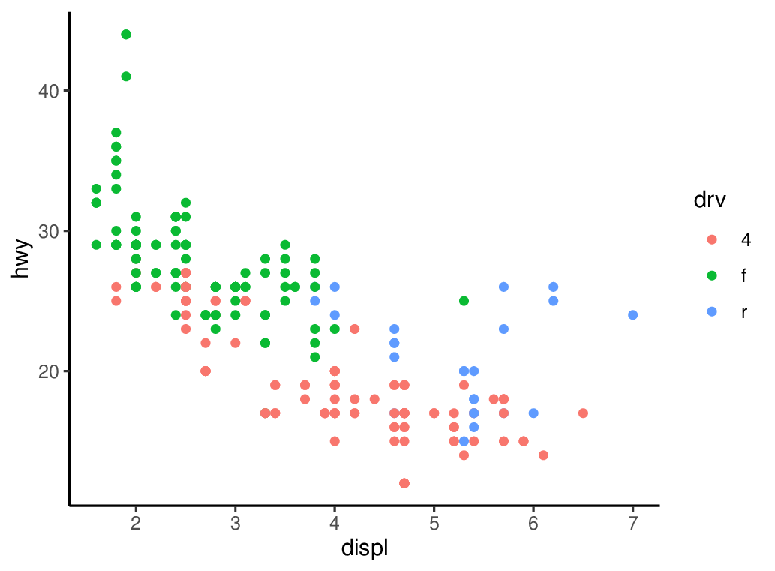
\includegraphics{fig/plot}
		\source{mpg, EUA}
		\notes{Mais Observações}
	\end{subfigure}
\end{figure}

\par Testando ref na Figura \ref{fig:test}
\lipsum[1-10]

\begin{figure}[!h]
	\begin{subfigure}{\linewidth}
		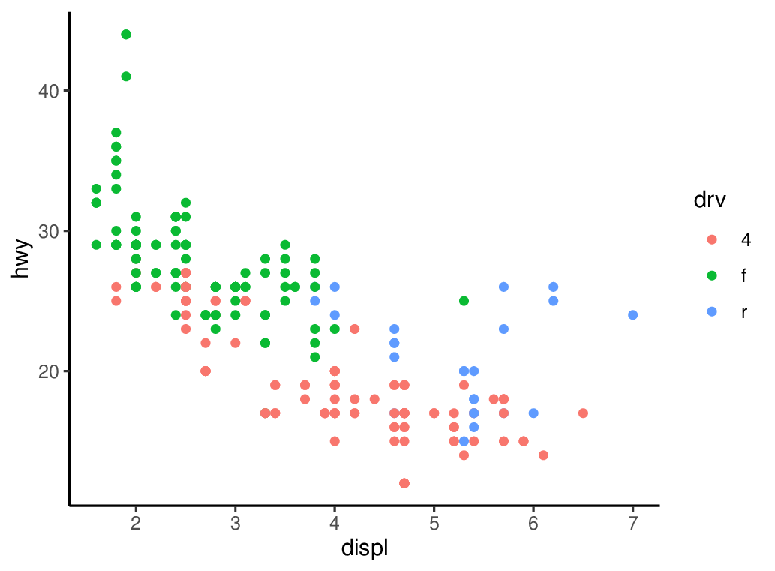
\includegraphics{fig/plot}
	\end{subfigure}
	\begin{subfigure}{\linewidth}
	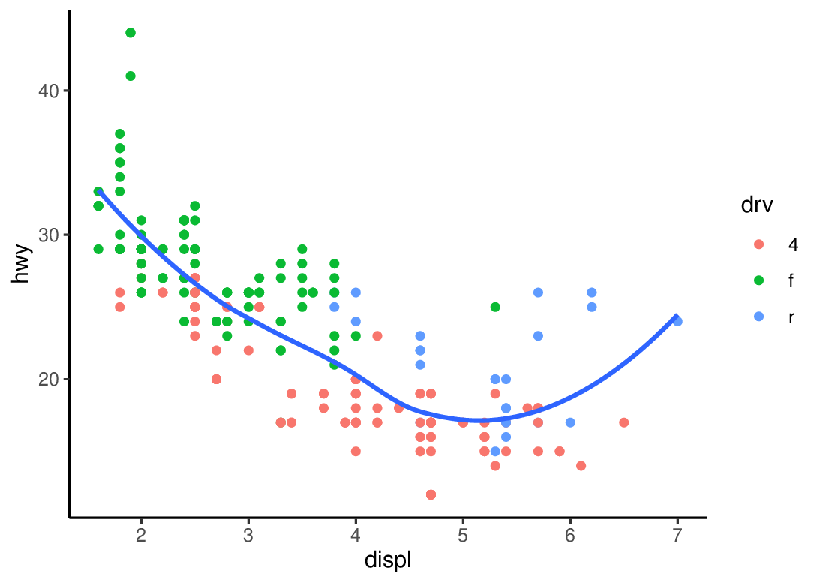
\includegraphics{fig/plot2}
	\end{subfigure}
	\begin{subfigure}{\linewidth}
		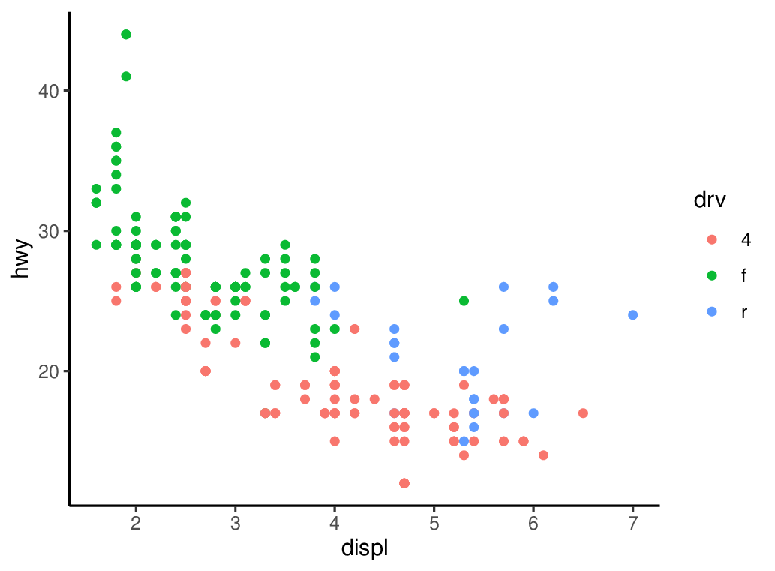
\includegraphics{fig/plot}
	\end{subfigure}
	\source{mpg, EUA}
\end{figure}

\lipsum[1-5]

\begin{figure}
\begin{subfigure}{\linewidth}
		\caption{Unica}\label{fig:single}
		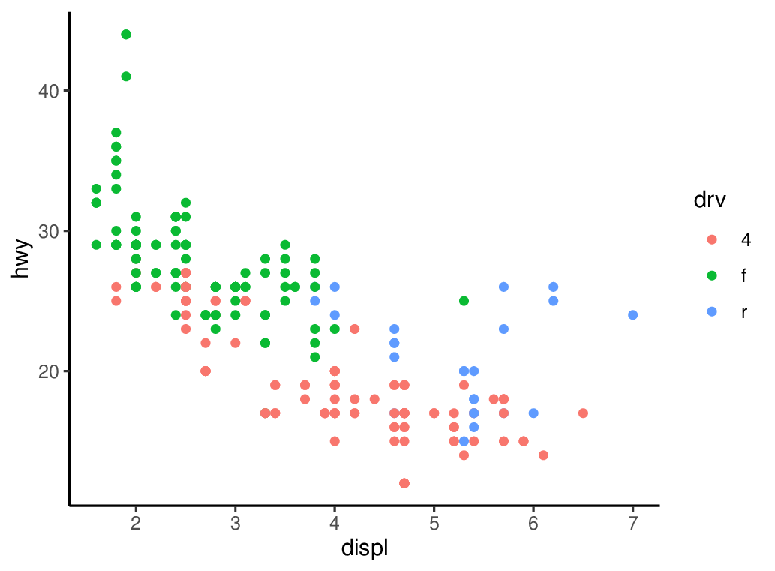
\includegraphics{fig/plot}
\end{subfigure}
\end{figure}

\par Testando a referência para a Figura \ref{fig:single}

\chapter{Titulo Capítulo 2}
	
\lipsum[1-6]

\par \ref{fig:figcap2}

\begin{figure}[!h]
	\begin{subfigure}{\linewidth}
		\caption{Titulo}\label{fig:figcap2}
		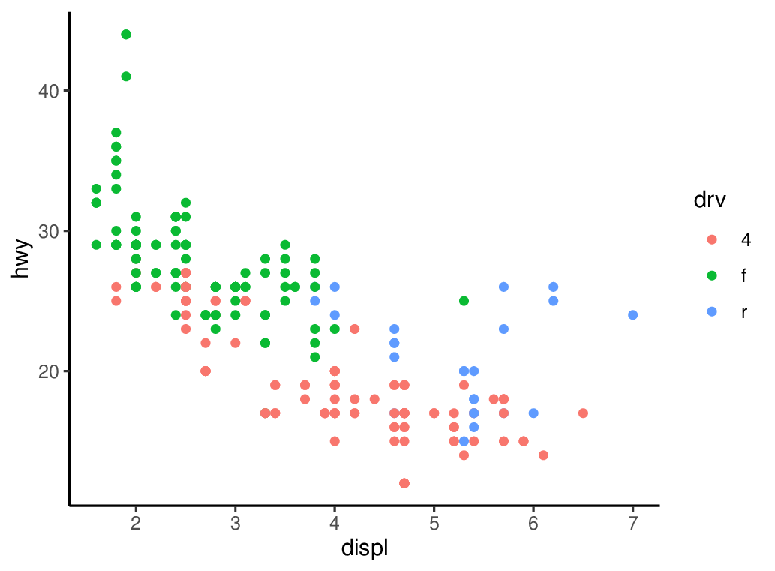
\includegraphics{fig/plot}
		\source{mpg, EUA}
		\notes{Mais observações}
	\end{subfigure}
	\begin{subfigure}{\linewidth}
		\caption{Titulo}
		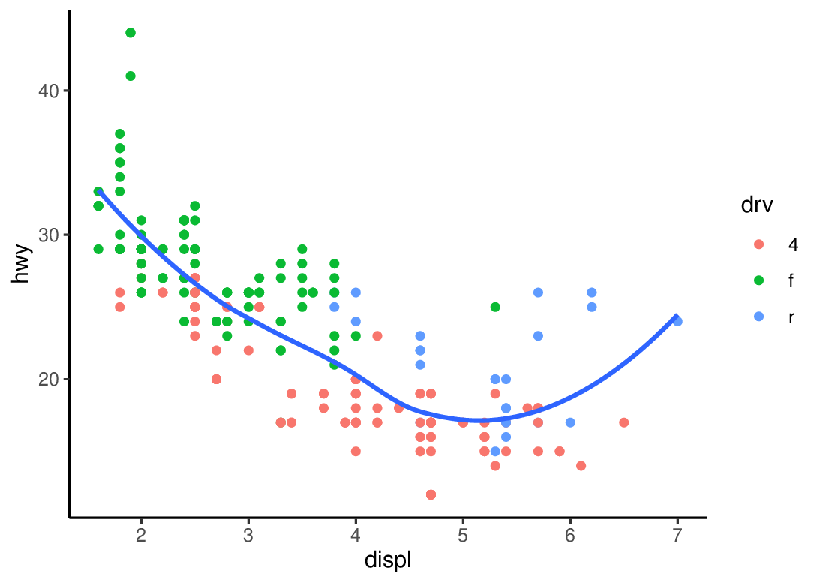
\includegraphics{fig/plot2}
		\source{mpg, EUA}
		\notes{Mais observações}
	\end{subfigure}
	\begin{subfigure}{\linewidth}
		\subcaption{Titulo}
		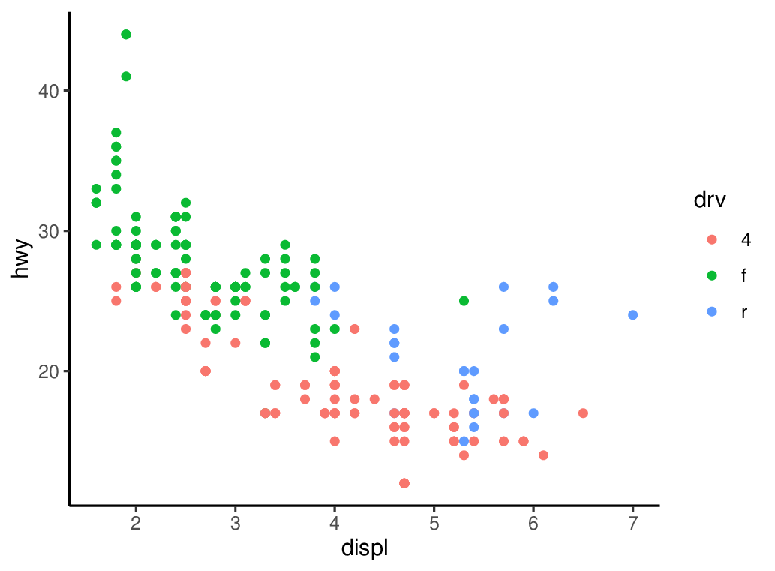
\includegraphics{fig/plot}
		\source{mpg, EUA}
		\notes{Mais Observações}
	\end{subfigure}
\end{figure}

\lipsum[1-10]

\begin{figure}
\begin{subfigure}{\linewidth}
		\caption{Unica}
		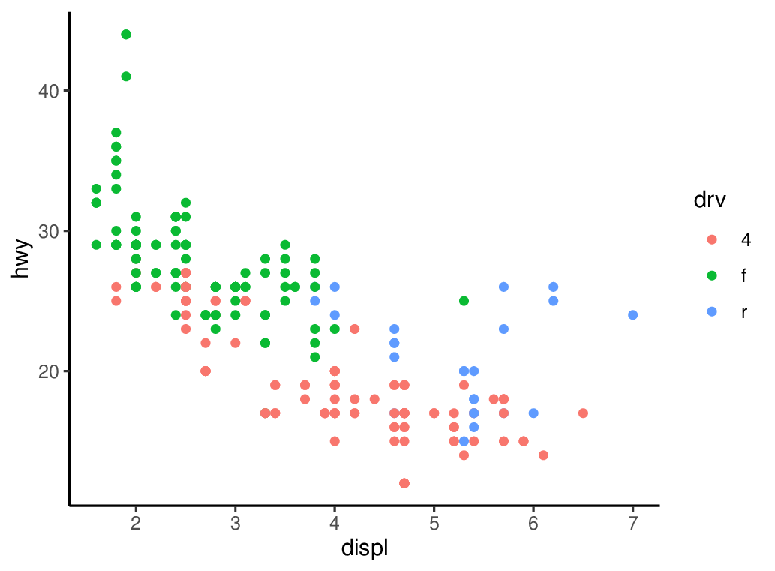
\includegraphics{fig/plot}
\end{subfigure}
\end{figure}
